\chapter{Detector Operation and Development}
\label{chap:RPC}

Resistive Plate Chambers (RPCs) are gaseous detectors operated in
avalanche or streamer mode, consisting of two parallel resistive
electrodes separated by a thin gas gap of the order of a few $\si{\milli\metre}$ and placed under a strong electric field of typically
several $\si{\kilo\volt\per\centi\metre}$. When a charged particle traverses the detector, it
ionises the gas and initiates an avalanche multiplication process.
The induced signal is collected by external readout strips,
providing fast timing information with a time resolution of
$\mathcal{O}(\SI{1}{\nano\second})$~\cite{AIELLI2004193,ARNALDI2000462,WILLIAMS2002183,BERTOLIN2009631,AIELLI200692,ZHANG2007278,ABBRESCIA2003137,AIELLI2013115}
and a coarse measurement of the particle position at the level of
$\mathcal{O}(\SI{1}{\centi\meter})$~\cite{CATTANI2012S6,ARNALDI200251}.
RPCs are characterised by a favourable combination of performance
and practicality, including robust operation and relatively simple
and cost-effective construction.

RPCs are widely used for triggering and timing applications, and are
also considered for high-granularity calorimetry concepts based on
particle-flow techniques, where fine segmentation and stable operation
are essential~\cite{PFA}. RPCs have therefore been widely deployed in
particle physics experiments such as ATLAS~\cite{Aad:2753039},
CMS~\cite{Shah_2020}, and ALICE~\cite{boss2012performance}
at CERN, as well as in astroparticle and neutrino experiments
including ARGO-YBJ~\cite{BARTOLI201547,BACCI2003110} and
Daya Bay~\cite{Ning_2013}. Beyond high-energy physics, RPC
technology has also been explored in applications such as time-of-flight
positron emission tomography (PET/CT) and volcano muon tomography
(TOMUVOL)~\cite{Crloganu2012TowardsAM}.

In addition to the physics analysis presented in this thesis,
the author has been involved in several activities related to RPC
detectors. These include the development of automated tools for
monitoring RPC performance using Detector Control System (DCS)
data in the ATLAS experiment, as well as participation in studies
related to the Phase-II upgrade of the RPC system.
In parallel, an independent detector R\&D study was carried out
to investigate improvements in the design of large-area glass RPC
chambers.

\section{RPC operation and monitoring in ATLAS}

The stable operation of RPC detectors is essential for the
performance of the ATLAS muon spectrometer. Variations in detector
conditions, such as changes in high voltage, gas flow, temperature
or humidity, can affect the detector response and therefore need to
be continuously monitored. The Detector Control System (DCS)
provides access to these parameters, allowing a detailed study of
the detector behaviour during data taking~\cite{DCS_EPJConf_2025,DCS_CDS_1564291,DCS_JPhysConfSer_2012}.

To facilitate such studies, an automated framework was developed to
retrieve and analyse RPC DCS data in an offline environment. The
framework combines luminosity information with detector parameters,
including the gap current ($I_{\mathrm{gap}}$), high voltage, gas
flow, temperature and relative humidity. The data are processed on
a run-by-run basis, enabling the evolution of detector performance
to be tracked over time.

The monitored observables are exploited in two complementary ways.
For quantities directly related to detector response, such as the
gap current, their dependence on the instantaneous luminosity is
studied. Since the gap current is expected to scale with the particle
flux, a linear relationship between $I_{\mathrm{gap}}$ and the
instantaneous luminosity is assumed, and the corresponding slope is
used as a measure of detector behaviour.
For observables describing detector conditions, including the high
voltage, gas flow, temperature and relative humidity, the average
value within each run is evaluated. The evolution of these
run-averaged quantities provides a direct probe of the stability of
the detector operating conditions over time. These two approaches are
illustrated in Figure~\ref{fig:rpc_monitoring_overview}.

\begin{figure}[htbp]
    \centering
    \begin{subfigure}{0.48\textwidth}
        \centering
        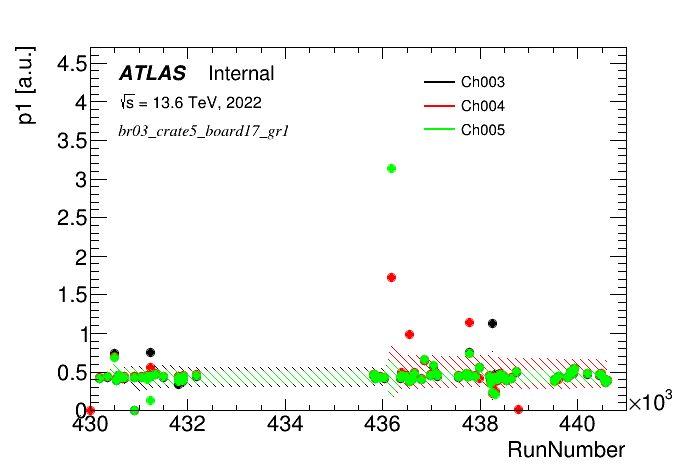
\includegraphics[width=\linewidth]{figures/RPC_main/p1_br03_crate5_board17_gr1.png}
        \caption{Slope of $I_{\mathrm{gap}}$ vs luminosity as a function of run number.}
        \label{fig:rpc_igap_slope}
    \end{subfigure}
    \hfill
    \begin{subfigure}{0.48\textwidth}
        \centering
        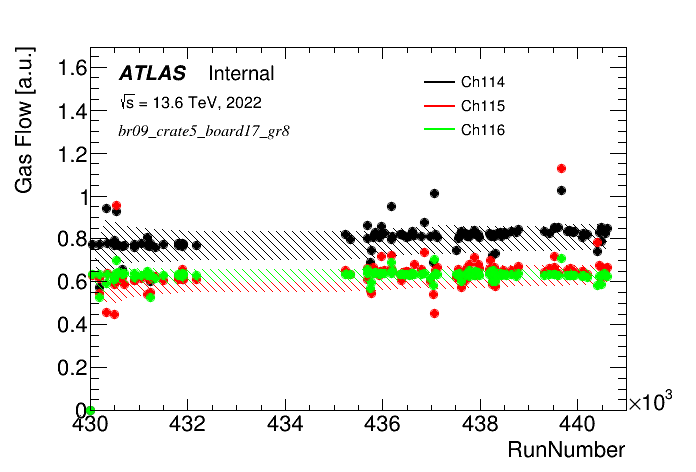
\includegraphics[width=\linewidth]{figures/RPC_main/gasflow_br09_crate5_board17_gr8.png}
        \caption{Average gas flow per chamber as a function of run number.}
        \label{fig:rpc_gasflow_trend}
    \end{subfigure}
    \caption{
    Monitoring of RPC detector behaviour using DCS observables.
    Detector response characterised by the dependence of gap
    current on luminosity (left) and stability of detector conditions
    illustrated by the evolution of the gas flow (right).
    }
    \label{fig:rpc_monitoring_overview}
\end{figure}

To identify anomalous detector behaviour, a statistical estimator is
defined to quantify deviations of monitored observables with respect
to their expected behaviour. For a given observable $x$ in a given run,
the estimator is constructed as
\begin{equation}
S = \frac{x - \mu}{\sigma},
\end{equation}
where $\mu$ and $\sigma$ denote the mean value and standard deviation
evaluated from a reference set of previous runs.

This normalised deviation provides a unified framework to identify
both local fluctuations and long-term drifts in detector behaviour.
Large values of $|S|$ indicate significant deviations from the
expected performance and may point to potential issues in detector
operation. The time evolution of the estimator for representative observables,
such as the P1 current and high voltage, is shown in
Fig.~\ref{fig:rpc_anomaly_detection}. Distinct anomaly patterns are
observed, including isolated spikes and gradual trends over multiple
runs. The method is therefore sensitive to different classes of
anomalies and provides a robust tool for monitoring RPC performance
over time.

\begin{figure}[htbp]
    \centering
    \begin{subfigure}{0.48\textwidth}
        \centering
        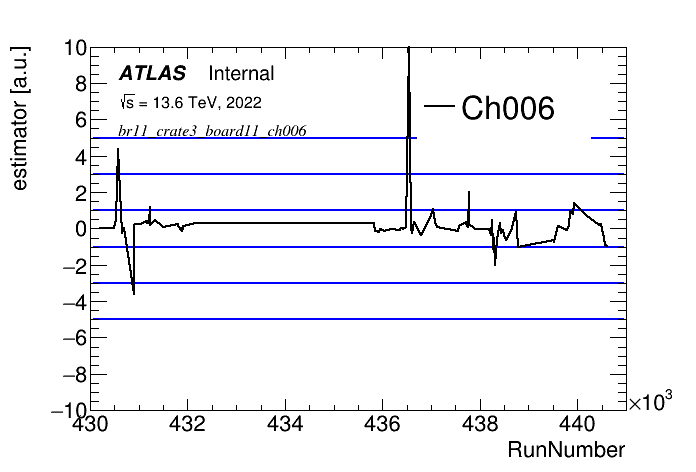
\includegraphics[width=\linewidth]{figures/RPC_main/trend_p1_br11_crate3_board11_ch006.png}
        \caption{Time evolution of the estimator $S$ derived from the slope of $I_{\mathrm{gap}}$ vs luminosity.}
    \end{subfigure}
    \hfill
    \begin{subfigure}{0.48\textwidth}
        \centering
        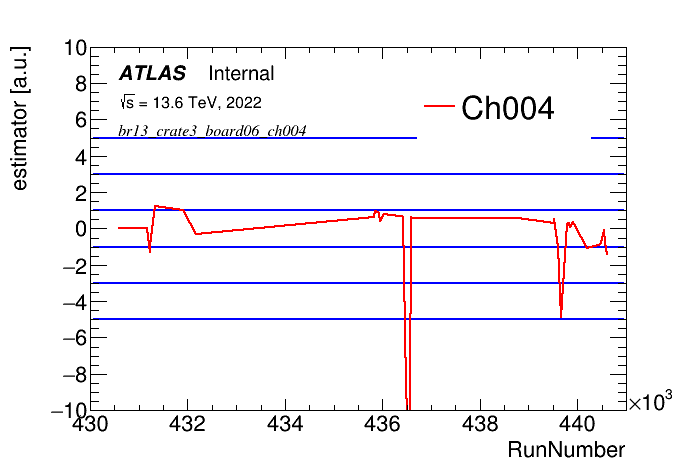
\includegraphics[width=\linewidth]{figures/RPC_main/trend_HV_br13_crate3_board06_ch004.png}
        \caption{Time evolution of the estimator $S$ derived from the applied high voltage.}
    \end{subfigure}
    \caption{
    Time evolution of the normalised deviation estimator $S$ for
    representative RPC observables as a function of run number.
    The estimator is constructed for different input quantities,
    including the slope of $I_{\mathrm{gap}}$ vs luminosity (left) and
    the high voltage (right), and provides a unified measure of deviations
    from the expected detector behaviour. Variations in $S$ reflect
    changes in detector response or operating conditions and are
    used to identify anomalous behaviour.
    }
    \label{fig:rpc_anomaly_detection}
\end{figure}

The full analysis chain has been automated, enabling new runs to be
processed as soon as they become available. The results are
summarised and visualised through a dedicated webpage~\cite{ATLAS_RPC_OfflineFW_Web}, providing a
compact overview of RPC performance over time. This framework allows
a quasi-real-time monitoring of detector conditions and supports
the identification of potential issues during data taking.
The author is responsible for the development of this framework and its
application to the analysis of Run~3 data as his qualification task.

\section{RPC phase-II upgrade studies for HL-LHC}

The HL-LHC will significantly increase the
instantaneous luminosity delivered to the ATLAS detector, leading to
higher particle rates and more demanding operating conditions for the
muon trigger system.
The current RPC system is subject to several limitations under these
conditions. The rate capability of the existing chambers is of the
order of $\mathcal{O}(100~\mathrm{Hz/cm^2})$, and long-term operation
at high luminosity may lead to detector ageing and a reduction in
efficiency. In addition, the presence of support structures introduces
regions of reduced acceptance.

To address these limitations, an upgrade of the RPC system is foreseen~\cite{CDS2285580,CDS2692929}. 
In the barrel inner (BI) region, a new detector layout is introduced as illustrated in Figure~\ref{fig:rpc_bi_layout}.
The new layout features three RPC triplets corresponding to a total of nine gas
gaps, thereby significantly increasing the trigger redundancy. In
addition, the gas-gap thickness is reduced from approximately
$2~\si{\milli\metre}$ to $1~\si{\milli\metre}$, enabling improved rate
capability and mitigating ageing effects under high-rate HL-LHC
conditions. The detector layout is further optimised to reduce
acceptance gaps and improve overall coverage.
These improvements are expected to significantly enhance the trigger
performance, with simulation studies indicating an increase in the
trigger efficiency from approximately 70\% to 90\% in the affected
regions.

\begin{figure}
    \centering
    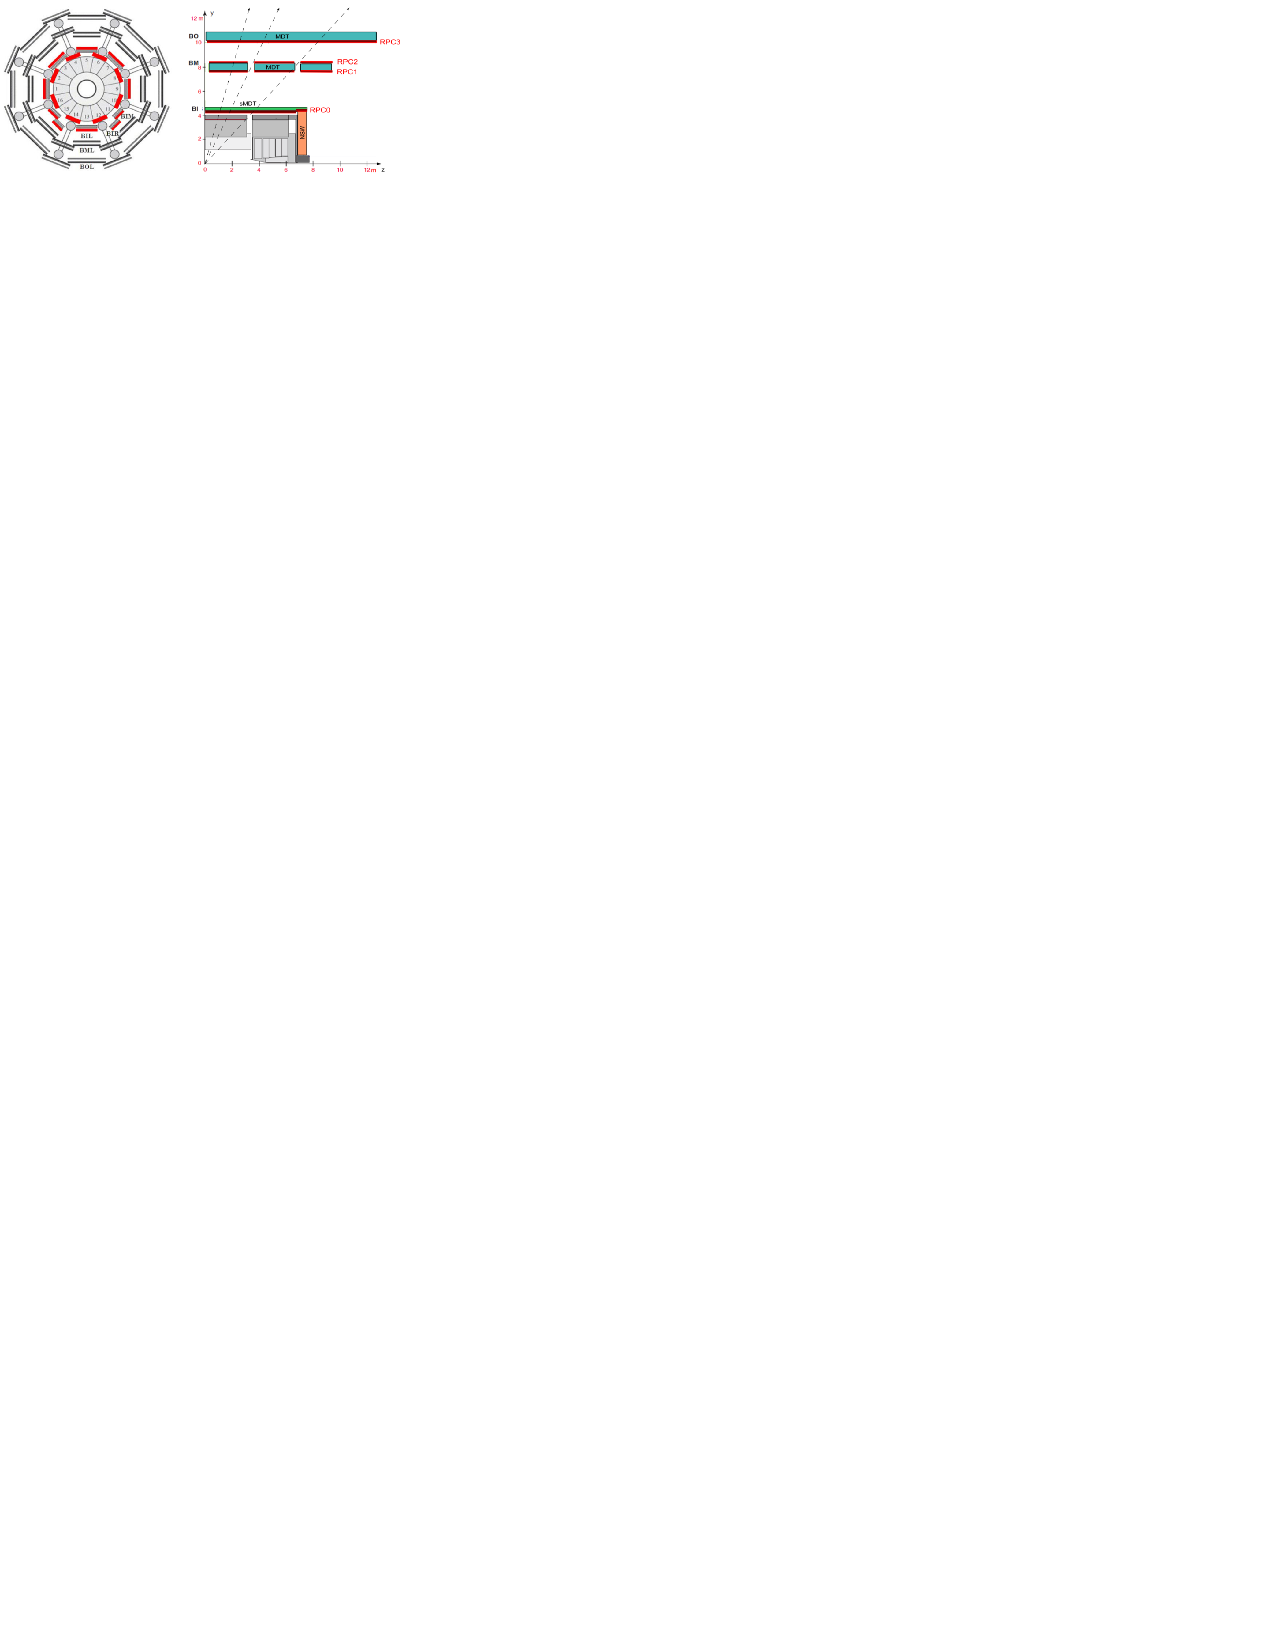
\includegraphics[width=0.72\textwidth]{figures/RPC_main/phaseII_layout.pdf}
    \caption{
    Layout of the ATLAS muon spectrometer highlighting the RPC system.
    x--y view showing the existing RPC chambers (dark grey) and
    the additional RPC layers (red) foreseen for the upgrade (left).
    R--z view of a quarter of the detector, indicating the
    location of the new RPC0 layer in the inner barrel region (right).
    Taken from Ref.~\cite{NIMA2024BI_RPC_ReadoutPanels}.
    }
    \label{fig:rpc_bi_layout}
\end{figure}

In view of the large-scale production required for the Phase-II
upgrade, ensuring consistent detector quality and stability is of
central importance. This involves both the control of fabrication
precision and the validation of detector performance through
conditioning procedures.
In this context, studies related to the pre-production of readout
panels and the conditioning of RPC gas gaps were carried out.

The readout panel constitutes a fundamental component of the RPC
detector unit, with each singlet consisting of one gas gap and two
readout panels. Given the large number of panels required for the
Phase-II upgrade, strict quality control and mechanical precision
are essential to ensure uniform detector performance.
Pre-production studies of readout panels focus on the validation of fabrication procedures and the
assessment of panel quality. The panel construction involves the
assembly of layered structures, for which uniform pressure and glue
distribution are required to achieve stable mechanical properties as illustrated in Figure~\ref{fig:rpc_panel_fabrication}. 

\begin{figure}[htbp]
    \centering
    \begin{subfigure}{0.48\textwidth}
        \centering
        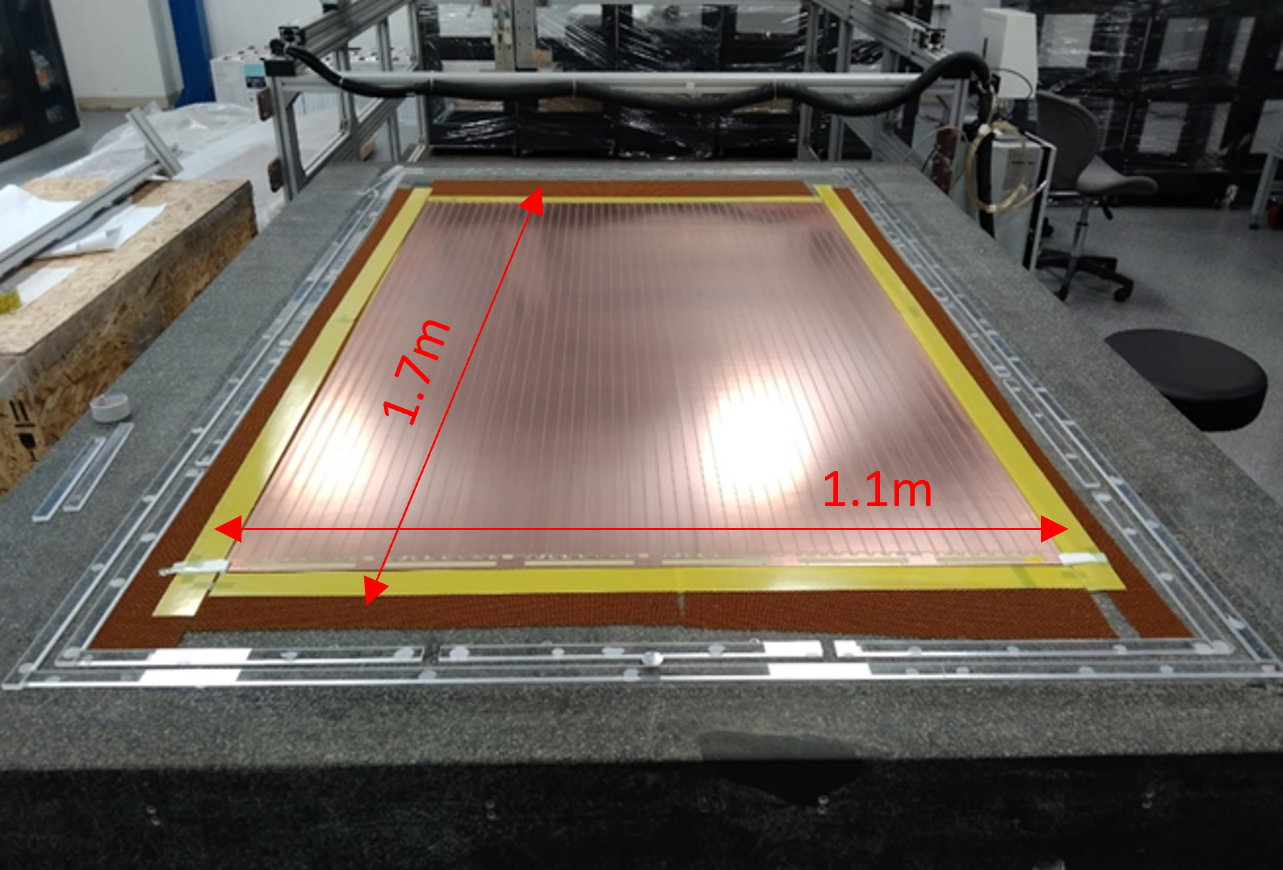
\includegraphics[width=\linewidth]{figures/RPC_main/pcb_surface.png}
        \caption{Preparation of the strip panel surface.}
        \label{fig:rpc_panel_surface}
    \end{subfigure}
    \hfill
    \begin{subfigure}{0.48\textwidth}
        \centering
        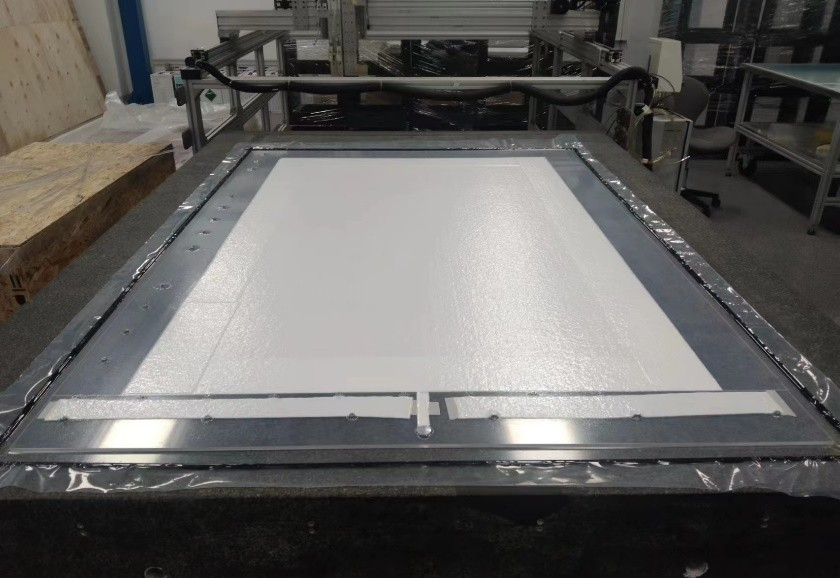
\includegraphics[width=\linewidth]{figures/RPC_main/pcb_pressing.jpg}
        \caption{Assembly under vacuum pressure.}
        \label{fig:rpc_panel_pressing}
    \end{subfigure}

    \caption{
    Fabrication procedure of the RPC readout panel. The panel is
    constructed by assembling PCB layers with a honeycomb core using
    adhesive. A vacuum-assisted pressing system is employed to apply
    uniform pressure during curing, ensuring homogeneous glue
    distribution and reducing local deformations. This step is
    essential for achieving stable mechanical properties and good
    thickness uniformity of the panel.
    }
    \label{fig:rpc_panel_fabrication}
\end{figure}

A key quality parameter is the thickness uniformity (flatness) of the
panels. The flatness is defined as the maximum variation in thickness
measured across the panel surface and is required to be less than
$\SI{100}{\micro\metre}$ within a local region of
$\sim 7\times7~\si{\centi\metre^2}$. Dedicated measurements were
performed to verify that the produced panels satisfy this requirement,
as illustrated in Figure~\ref{fig:rpc_panel_flatness}.

\begin{figure}[htbp]
    \centering
    \begin{subfigure}{0.48\textwidth}
        \centering
        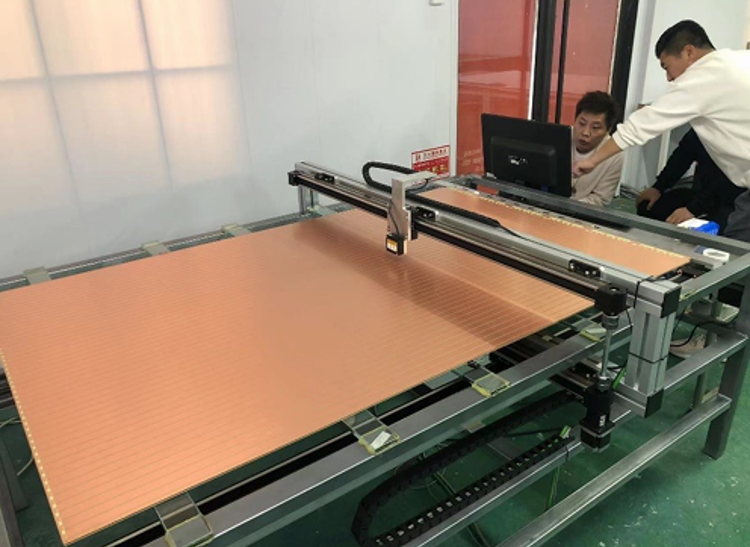
\includegraphics[width=\linewidth]{figures/RPC_main/pcb_testing.png}
        \caption{Automated thickness scanning setup.}
        \label{fig:rpc_panel_scan}
    \end{subfigure}
    \hfill
    \begin{subfigure}{0.48\textwidth}
        \centering
        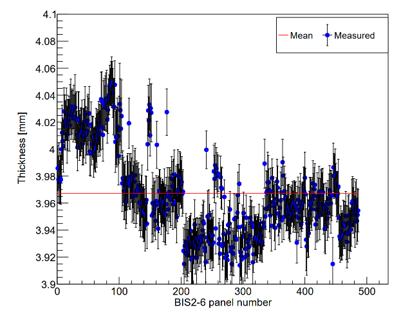
\includegraphics[width=\linewidth]{figures/RPC_main/pcb_result.png}
        \caption{Measured thickness distribution.}
        \label{fig:rpc_panel_result}
    \end{subfigure}

    \caption{
    Thickness measurement and flatness evaluation of the readout panel.
    The panel thickness is measured using a motorised scanning system
    equipped with a laser distance sensor, which performs point-by-point
    measurements over a predefined grid.
    }
    \label{fig:rpc_panel_flatness}
\end{figure}

In addition to the validation of detector components prior to mass
production, conditioning tests of assembled RPC gas gaps are
performed to ensure stable operation under high-voltage conditions.
These tests are carried out at the GIF++ facility at CERN, which
provides a controlled irradiation environment to emulate the
high-rate conditions expected at the HL-LHC.
The conditioning procedure involves gradually increasing the applied high voltage
while monitoring the detector currents and stability over time.
Initial and final high-voltage scans, together with continuous
current monitoring, are used to evaluate the evolution of the
detector response.
Further details of this study are presented in Appendix~\ref{sec:rpc_gifpp_conditioning}.

\section{RPC chamber design optimisation}
\label{sec:rpc_optimisation}

In parallel to the ATLAS-related detector activities described above,
an independent detector R\&D study was carried out to optimise the
internal design of large-area glass RPC chambers, based on work
published in Ref.~\cite{Mao2021JINST_RPC}. A key design challenge in
such detectors is the use of spacers: while spacers are required to
maintain a uniform gas gap and mechanical stability, they also
introduce inactive regions and locally perturb the gas flow. The
detector design must therefore balance several competing requirements,
including minimising dead area, preserving gas-gap uniformity,
maintaining sufficiently homogeneous gas circulation, and ensuring a
construction procedure that remains simple and robust.

To address this, an optimisation of the spacer configuration was
performed for a $1\times1~\si{m^2}$ glass RPC. Two layouts were
considered: a reference design with an aligned $10\times10$ grid of
100 spacers, and an optimised shifted-spacer design with 76 spacers.
Both configurations are illustrated in Figure~\ref{fig:rpc_spacer_layouts}.
The comparison was carried out using coupled multi-physics simulations
in \textsc{COMSOL}, combining gas-flow, structural-mechanics and
electrostatic calculations under realistic operating conditions. The
study focused on gas-flow homogeneity, vorticity, electrode
deformation, and electric-field stability.

\begin{figure}[htbp]
    \centering
    \begin{subfigure}{0.45\textwidth}
        \centering
        
\includegraphics[width=\linewidth]{RPC_images/Drawing1.png}
        \caption{Reference spacers configuration.}
    \end{subfigure}
    \hfill
    \begin{subfigure}{0.45\textwidth}
        \centering
        
\includegraphics[width=\linewidth]{RPC_images/Drawing2.png}
        \caption{Shifted spacers configuration.}
    \end{subfigure}
    \caption{
    Comparison of the two spacer layouts considered in the optimisation
    study for a $1\times1~\si{m^2}$ glass RPC chamber.
    }
    \label{fig:rpc_spacer_layouts}
\end{figure}

The optimised configuration improves the uniformity of the gas flow,
with the relative velocity dispersion reduced from 20.3\% to 17.5\%,
and slightly lowers the bulk vorticity in the chamber. At the same
time, the deformation of the gas gap remains at the sub-percent level,
indicating that the reduction in spacer number does not compromise
mechanical stability. A summary of the main performance metrics is
given in Table~\ref{tab:rpc_opt_summary}. Prototype measurements with
cosmic muons show that both designs reach efficiency plateaus above
95\% as illustrated in Figure~\ref{fig:rpc_efficiency_comparison}, 
demonstrating that the shifted-spacer layout preserves detector
performance while reducing the inactive area associated with spacers.

\begin{table}[htbp]
    \centering
    \begin{tabular}{lcc}
        \hline
        Metric & Reference & Shifted \\
        \hline
        Number of spacers & 100 & 76 \\
        Relative velocity dispersion $\sigma_v/\bar{v}$ & 20.3\% & 17.5\% \\
        Deformation uniformity $\sigma_d/\bar{d}$ & 0.25\% & 0.42\% \\
        Efficiency plateau & $>95\%$ & $>95\%$ \\
        \hline
    \end{tabular}
    \caption{
    Summary of the main simulation and prototype-performance metrics for
    the two spacer configurations.
    }
    \label{tab:rpc_opt_summary}
\end{table}

\begin{figure}[htbp]
    \centering
    
\includegraphics[width=0.72\textwidth]{RPC_images/Efficiency.png}
    \caption{
    Detection efficiency as a function of applied high voltage for the
    reference and shifted-spacer RPC prototypes. Both configurations
    reach efficiency plateaus above 95\%.
    }
    \label{fig:rpc_efficiency_comparison}
\end{figure}

Overall, the study shows that careful optimisation of the spacer
layout can reduce the number of spacers by about 24\% while preserving
stable operation and high detection efficiency. Detailed descriptions
of the simulation framework, prototype construction and cosmic-ray
test setup are provided in Appendix~\ref{chap:rpc_appendix}.